% ========================================
% CHAPTER 3: RELATED WORK (WHAT WAS PREVIOUSLY DONE)
% ========================================
\chapter{Related Work}


% ========================================
% SECTION 3.1: ARCHITECTURAL APPROACHES FOR LONG CONTEXT MODELING
% ========================================
\section{Architectural Approaches for Long Context Modeling}

Review of prior research that addressed long contexts through architectural innovations (e.g., Recurrent Memory Transformer (RMT), Longformer).
Note that while these methods reduce computation, they often suffer from a decline in performance on long contexts.

% Insbesondere weisen wir auf den wunderbaren Artikel von \textcite{Edmonds:1965} und auf~\cite{GareyJohnson:1979} für weitere Hintergründe.


% ========================================
% SECTION 3.2: SOFT PROMPTING AND CONTEXT DISTILLATION TECHNIQUES
% ========================================
\section{Soft Prompting and Context Distillation Techniques}

Summary of related soft prompt methods like GIST and AutoCompressor that utilize an LLM to compress context into special tokens or summary vectors.
Highlighting that these methods are often limited to compressing short prompts or require complex recursive training.


% ========================================
% SECTION 3.3: THE IN-CONTEXT AUTOENCODER (ICAE) FRAMEWORK
% ========================================
\section{The In-Context Autoencoder (ICAE) Framework}

Introduction of ICAE \cite{ge_-context_2024} as the most closely related study, leveraging an LLM to compress long context into memory slots that are conditioned on by the decoder (the frozen LLM itself).

\begin{figure}[hbt]
  \centering
  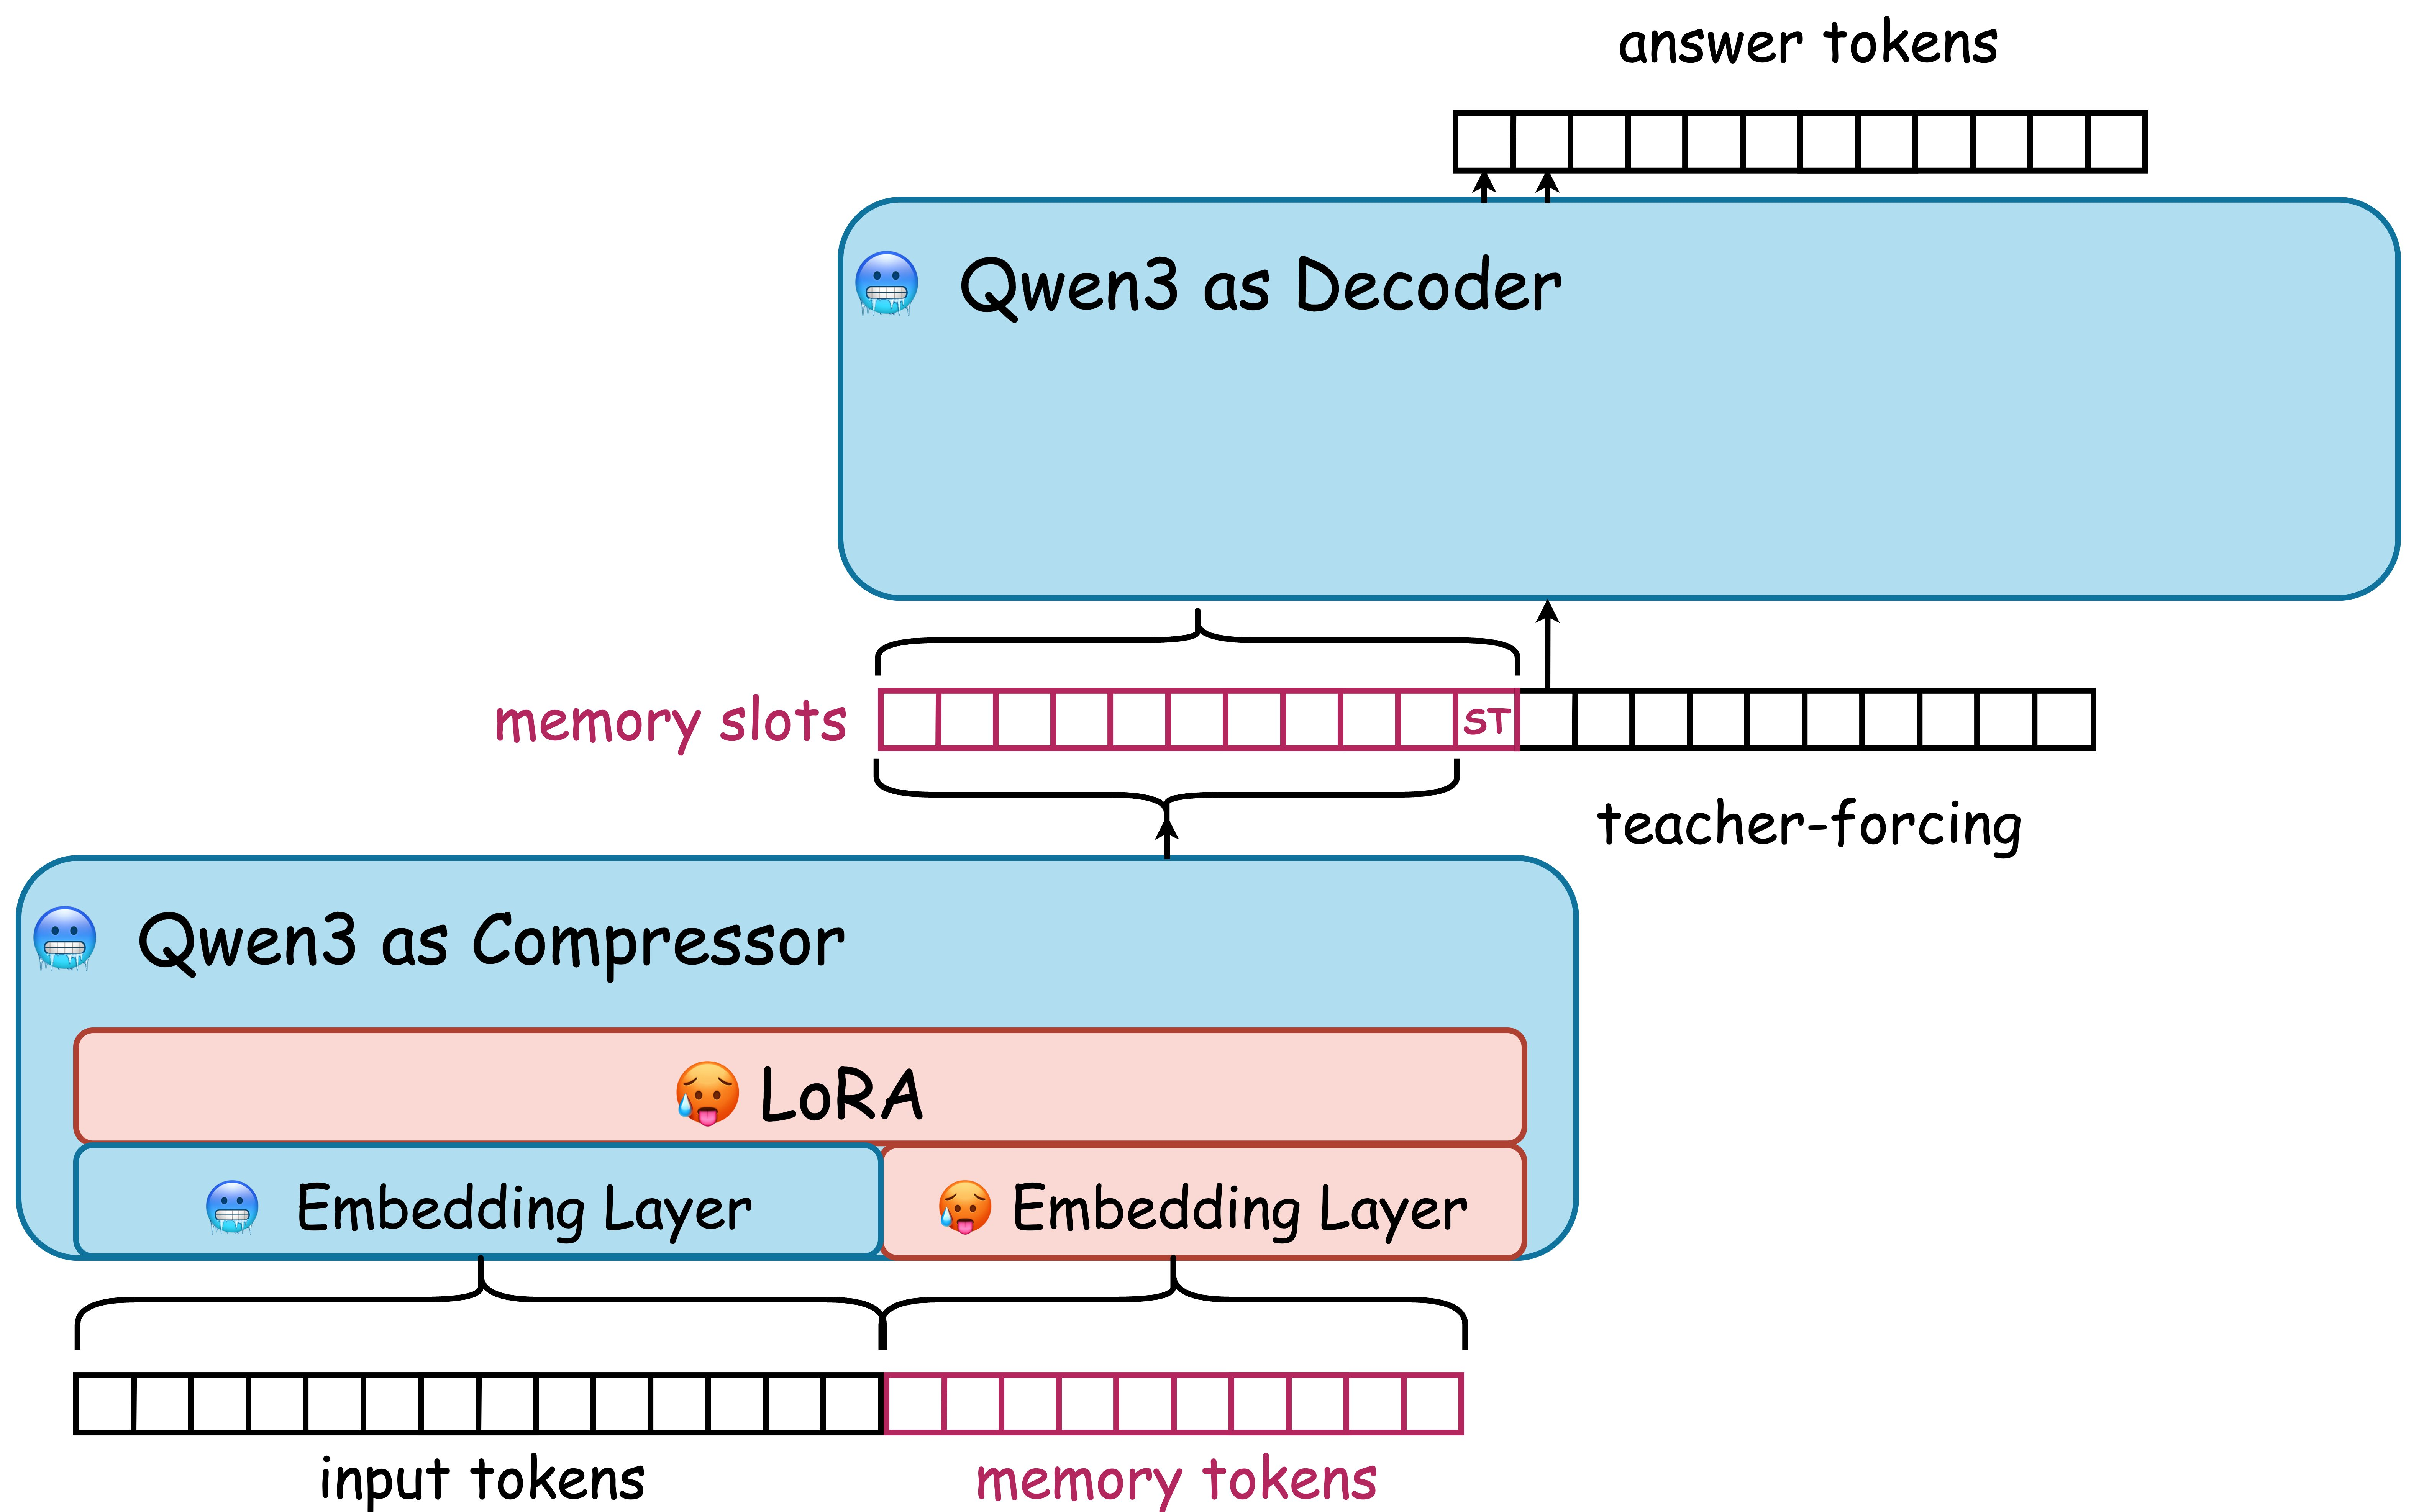
\includegraphics[width=0.8\textwidth]{graphs/icae.jpeg}
  \caption{In-Context Autoencoder (ICAE) framework architecture}
  \label{fig:icae}
\end{figure}
